%%%%%%%%%%%%%%%%%%%%%%%%%%%%%%%%%%%%%%%%%%%%%%%%%%%%%%%%%%%%%%%%%%%%%%%
%%%%%%%%%%%%%%%%%%%%%%%%%%%%%%%%%%%%%%%%%%%%%%%%%%%%%%%%%%%%%%%%%%%%%%%
%%%%%                                                                 %
%%%%%     02_background.tex                                           %
%%%%%                                                                 %
%%%%% Author:      <author>                                           %
%%%%% Created:     <date>                                             %
%%%%% Description: <description>                                      %
%%%%%                                                                 %
%%%%%%%%%%%%%%%%%%%%%%%%%%%%%%%%%%%%%%%%%%%%%%%%%%%%%%%%%%%%%%%%%%%%%%%
%%%%%%%%%%%%%%%%%%%%%%%%%%%%%%%%%%%%%%%%%%%%%%%%%%%%%%%%%%%%%%%%%%%%%%%

\chapter{Background}
\label{chapter:background}

\section{PULP (Parallel Ultra-Low-Power Processing-Platform)}

The \gls{PULP} is a combined effort of ETH Zurich and the University of Bologna
with the help of Politechnico di Milano to create an efficient ultra-low-power
many-core platform. The \gls{PULP} project has been running for two years and
during this time several tape outs have been done already, the most important
include pulp1 and pulp2 which represent the state of the \gls{PULP} system at
that time.

\gls{PULP} will finally consist of several clusters with independent clock and
power domains. Within each cluster there are several simple \gls{RISC} cores
that perform the computations.

Currently we concentrate on the cluster level which is why we only work with one
cluster. In Figure~\ref{fig:pulp_overview}, a typical \gls{PULP} system with one
cluster is shown. In the top level, outside the cluster, there is a big L2
\gls{RAM} that contains the program code for the cores in the system.
\gls{PULP} can either work as an accelerator for a host or run in standalone
mode where it boots from its internal \gls{ROM} and loads an application from an
external flash. The system also provides several peripherals like \gls{SPI} and
\gls{UART} which can be used to communicate with the outside world.

Alongside the cores in the cluster, there is a multi-banked \gls{TCDM} that
uses word-level interleaving to minimize contentions between accesses from the
different cores. If there is no contention, the cores can load or store a word
in the \gls{TCDM} in a single cycle. Typically the number of banks is twice the
number of cores per cluster, so for a system with four cores as in
Figure~\ref{fig:pulp_overview} eight \gls{TCDM} banks are used.

The \gls{TCDM} inside the cluster is divided into \gls{SRAM} and \gls{SCM} based
memories. The \gls{SCM} memory is usually much smaller in storage capacity
compared to the \gls{SRAM} while being much bigger in terms of area. The big
advantage of using an \gls{SCM} is that the \gls{SCM} is able to work with lower
voltages where conventional \gls{SRAM} does not work properly anymore. This
allows us to lower the voltage of the whole cluster when the \gls{SRAM} is not
used.

For the 4-core PULP system the cores within each cluster share a common 4-way
associative instruction cache which is connected to the L2 \gls{RAM}. Sharing a
common instruction cache between the cores is done to reduce energy, because it
is often the case that all cores inside a cluster execute the same application
and thus most of the cache entries can be shared between them. This scheme makes
the whole cluster more efficient as a smaller instruction cache can be used
compared to four independent caches. To reduce access contention in this shared
setting, two methods are used. First a 128 bit wide L0 buffer is placed between
the cache and the core which holds the most recently used cache line.  This
buffer holds four instructions and thus the cores do not need to access the
instruction cache in every cycle.
Furthermore the cache is divided into four banks of 1 KB each which can be
accessed individually and thus contentions only arise when multiple cores need
to access the same cache bank.

\begin{figure}[htbp]
  \centering 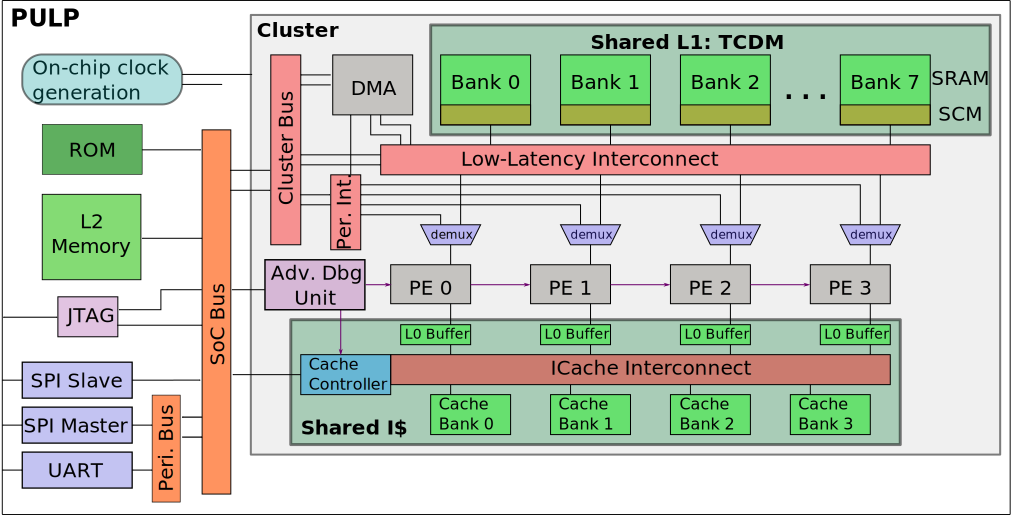
\includegraphics[width=0.9\textwidth]{./figures/PULP}
  \caption{PULP system overview.}
  \label{fig:pulp_overview}
\end{figure}

Until the beginning of this thesis \gls{PULP} was using a modified version of
the OR1200 OpenRISC core \cite{OR1200} that was created by the OpenRISC
community. During this thesis we switched the core to \orion, the core that we
developed solely for its use in \gls{PULP}.


\section{OR10N Core}

\orion is the OpenRISC core that replaces the previously used OR1200. \orion was
originally developed by Matthias Baer and Renzo Andri during a semester thesis
at ETHZ. It was already used in several chips, for example Sir10us
\cite{Sir10us} and \orion that were produced in 180 nm UMC technology and
successfully tested before we started integrating \orion into the \gls{PULP}
environment.

Prior to this thesis, the instruction set of \orion was enhanced with several
features that are not part of the OpenRISC specifications, specifically support
for hardware loops and auto-incrementing load and store operations, see
Section~\ref{sec:or10n_hwlp_prepost} for more details on the extensions.


\begin{figure}[htbp]
  \centering \includegraphics[width=0.9\textwidth]{./figures/or10n_overview}
  \caption{\orion general overview.}
  \label{fig:or10n_overview}
\end{figure}


\orion is based on a simple in-order four stage pipeline. In terms of core
energy efficiency an in-order single-issue processor design is the most
efficient \cite{azizi2010}. To achieve high \gls{IPC} values in such a core a
shallow pipeline with a low number of pipeline stages is important as this
reduces the number of possible data hazards.
The four pipeline stages of our \orion core are \gls{IF}, \gls{ID}, \gls{EX}
and \gls{WB}.

During the IF stage instructions get transferred from the instruction cache to
the core and the program counter is updated with the next value. If the
instruction cache can not immediately deliver the required instruction, the core
is stalled for the required amount of cycles.

The ID stage takes care of decoding instructions, performing accesses to the
register file and forwarding results to operands if they are needed in the next
cycle. Also the main control \glspl{FSM} reside in this stage.

The EX stage is the main computation stage in \orion. ALU and multiplication
operations are performed here and the results stored in the register file.
The address for a memory access is computed during the EX stage and sent to
the data memory interface.
If the address belongs to the \gls{TCDM} address space, data can be accessed in
a single cycle.
Otherwise a memory access will take multiple cycles and the core needs to be
stalled until the request has been served and the required data has been
delivered to the core.

During the \gls{WB} stage, the received data is multiplexed with \gls{SPR} data
and stored in the \gls{GPR}. The \gls{LSU} that is responsible for managing
memory accesses is part of the \gls{WB} stage and takes care of sign-extending
the received data and aligning it.
The \gls{SPR} that contains data that is important during the runtime of the
\gls{CPU}, is also part of the \gls{WB} stage. For example the arithmetic carry
and overflow flags are stored in the \gls{SPR} and can be accessed with
\instr{l.mfspr} instructions.

\orion uses a five port general-purpose register file with two write ports and
three read ports. One write port of the register file is used for ALU operations
exclusively, while the second write port is shared between SPR and memory
access. Two of the three read ports of the register file are used for normal \gls{ALU}
operations and memory accesses. The third read port is only used for two special
operations, namely the multiply-accumulate operation and register-register
store operations.

The final \orion core needs $44.5$ kGE area and achieves a clock period of
$2.23$ ns clock period in a UMC $65$ nm technology. The critical path in the
core is balanced between data memory address generation, the \gls{MAC} unit and
instruction fetch from the shared instruction cache.


\section{Compiler Support}

To write applications for the PULP platform we did not want to rely exclusively
on assembler as this makes development cumbersome and error-prone, instead C is
mainly used.
Thus to perform the translation from C to OpenRISC machine code a compiler is needed.
The OpenRISC community has already provided a port of \gls{GCC} to OpenRISC
which we reused for our system. But to get more performance and being able to
use our additional instructions, some changes to the compiler were needed to
actually emit those new instructions automatically. The researchers at
Politechnico di Milano did a port of the LLVM compiler to OpenRISC and added
support for our instruction set extensions to it.  This means that one can write
applications for PULP entirely in C and benefit from our \gls{ISA} extensions
automatically as there is full compiler support for it.

Writing parallel applications for a multi-core environment is difficult. To
simplify the development such applications, we ported OpenMP to our platform and
thus a programmer can take advantage of the constructs given by this framework.

%Eric Flamand has been working on adapting \gls{GCC} to the new instruction set
%that we have been developing. So our additional instructions are supported by
%both major compilers, \gls{GCC} and LLVM which allows us to make direct
%comparisons between the two.
%
%Both compilers are able to automatically emit code that uses the additional
%instructions and thus we can accelerate existing code without changing it.

%%% Local Variables: 
%%% mode: latex
%%% TeX-master: "../report_template"
%%% End: 
